\documentclass{book}
\usepackage{hyperref} % For hyperlinks
\usepackage{fancyhdr}  % For customizing headers and footers
\usepackage{titlesec}  % For customizing title formats
\usepackage{inconsolata}
\usepackage[]{graphics} % For using local images
\usepackage{graphics} % For using local images
\usepackage{epstopdf}

\usepackage{color}
\definecolor{bluekeywords}{rgb}{0.13,0.13,1}
\definecolor{greencomments}{rgb}{0,0.5,0}
\definecolor{redstrings}{rgb}{0.9,0,0}

\usepackage{listings}
\lstset{language=[Sharp]C,
  showspaces=false,
  showtabs=false,
  breaklines=true,
  showstringspaces=false,
  breakatwhitespace=true,
  escapeinside={(*@}{@*)},
  commentstyle=\color{greencomments},
  keywordstyle=\color{bluekeywords},
  stringstyle=\color{redstrings},
  basicstyle=\ttfamily
}
\title{.NET Interview Questions}
\author{Konstantin Milchev }
\date{}

% Globally center all chapter titles
\titleformat{\chapter}[display]
  {\normalfont\huge\bfseries\centering} % Format for the chapter title (centering)
  {} % Label (empty since you may be using \chapter* for no numbering)
  {0pt} % Space before the title
  {\Huge} % Format of the chapter title itself

  
% Configure fancyhdr
\pagestyle{fancy}      % Use fancy page style for default layout
\fancyhf{}             % Clear all header and footer fields
\fancyfoot[C]{\thepage} % Set page number at the bottom center by default
\renewcommand{\headrulewidth}{0pt} % Remove the header line
\setlength{\headheight}{0pt}       % Remove the height of the header
 
\begin{document}

% Title Page
\maketitle

% Use \clearpage to avoid blank pages
\clearpage

% Table of Contents
\tableofcontents

% Start of the pages
 
\newpage
% Include other files here
\chapter{Heap}
\section{Definition}
	A heap is a \textbf{binary} tree with two properties:
	\begin{itemize}
		\item Shape: Its shape must be complete. All of the nodes from all the levels must be filled, except the last one.
		\item Order: It must have all of its nodes in a specific order.
		\begin{itemize}
			\item \textbf{Min-Heap}: A heap's root node must have of its children be either smaller than or equal to it's children.
			\item \textbf{Max-Heap}: A heap's root node must have of its children be either greater than or equal to it's children.
		\end{itemize}
	\end{itemize}
\section{Basics}
	\begin{itemize}
		\item We can always have duplicates in a heap
		\item Heaps don't follow the binary search tree rule that the left node needs to be smaller than the right.
		\item No matter if we grow or shrink the heap, we must always maintain it's two properties
		\item It's used in a system scheduler where a priority queue will say which task should be executed next (task, item with highest priority will be dequeued from the heap)
	\end{itemize}
	\section{Storing a Heap}
	\begin{figure}[H]
		\centering
		\scalebox{0.40}
			{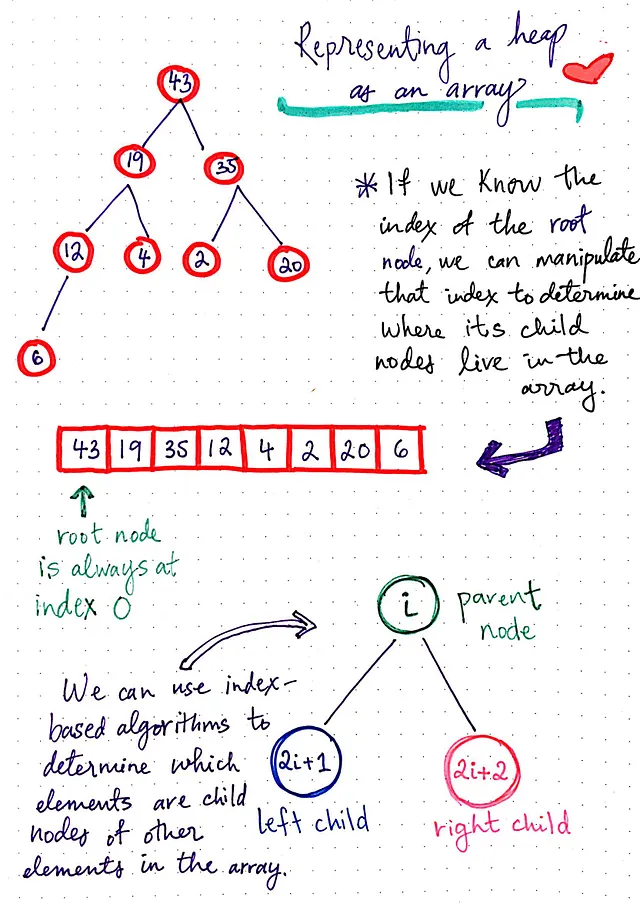
\includegraphics{images/heap_1}}
		\caption{Heap as an array structure}
	\end{figure}	
	
	\section{Getting the heap out of the Array}
	\begin{figure}[H]
		\centering
		\scalebox{0.40}
			{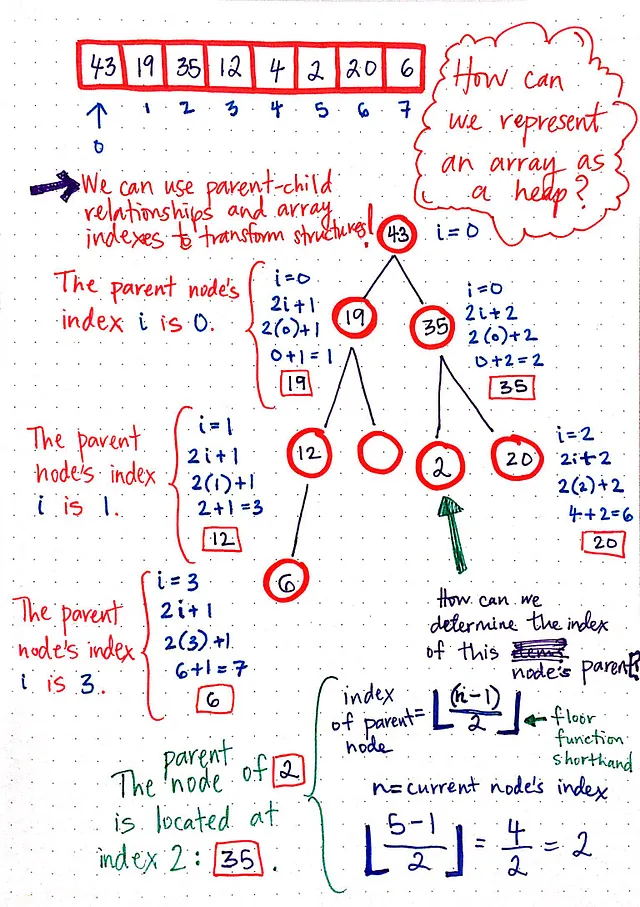
\includegraphics{images/heap_2}}
		\caption{Heap as an array structure}
	\end{figure}	
	
	\section{Heap Sort Algorithm}
		\begin{itemize}
			\item Improved Selection Sort with O(nlogn) time complexity
			\item buildMaxHeap()
			\item heapify()
		\end{itemize}

		
		\section{Techniques}
		\begin{itemize}
			\item If you see a top or lowest k being mentioned in the question, it is usually a signal that a heap can be used to solve the problem, such as in \textbf{Top K Frequent Elements.}
			\item Stack with one item
			\item Stack with two items
		\end{itemize}
		
	
	\section{Time complexity}
	
	\begin{center}
		\begin{tabular}{||c c||}
		\hline
		Operation & Complexity\\
		\hline\hline
		Find max/min & O(1)\\
		\hline
		Insert & O(log(n))\\
		\hline
		Remove & O(log(n))\\
		\hline
		Heapify(create a heap of a given array of elements) & O(1)\\
		\hline
			
		\end{tabular}
	\end{center}
	
	
	
	


\end{document}
